\documentclass[tikz]{standalone}

\usetikzlibrary{backgrounds}
\usepackage{xcolor}

% choose which set of colors to use
\definecolor{bgColor}{HTML}{ffffff}
\definecolor{fgColor}{HTML}{14181e}

% \definecolor{bgColor}{HTML}{14181e}
% \definecolor{fgColor}{HTML}{ffffff}

\begin{document}
	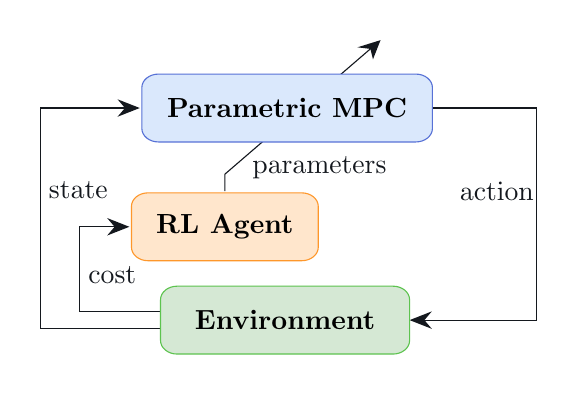
\begin{tikzpicture}[x=0.75pt,y=0.75pt,yscale=-0.8175,xscale=1, background rectangle/.style={fill=bgColor}, show background rectangle]
		% Straight Lines
		\draw [fgColor] (140,89) -- (140,79) -- (212.93,2.18);
		\draw [fgColor] (109,160) -- (70,160) -- (70,110) -- (91,110);
		\draw [fgColor] (109,170) -- (51,170) -- (51,40) -- (96,40);
		\draw [fgColor] (240,40) -- (290,40) -- (290,165) -- (232,165);

		% Arrows
		\draw [fill=fgColor, shift={(215, 0)},   rotate=133.51, draw opacity=0] (10.72,-5.15) -- (0,0) -- (10.72,5.15) -- (7.12,0) -- cycle;
		\draw [fill=fgColor, shift={(94,  110)}, rotate=180,    draw opacity=0] (10.72,-5.15) -- (0,0) -- (10.72,5.15) -- (7.12,0) -- cycle;
		\draw [fill=fgColor, shift={(99,  40)},  rotate=180,    draw opacity=0] (10.72,-5.15) -- (0,0) -- (10.72,5.15) -- (7.12,0) -- cycle;
		\draw [fill=fgColor, shift={(229, 165)}, rotate=360,    draw opacity=0] (10.72,-5.15) -- (0,0) -- (10.72,5.15) -- (7.12,0) -- cycle;

		% Rounded Rect
		\draw [color={rgb,255:red,254;green,151;blue,43}, fill={rgb,255:red,255;green,230;blue,204}] (95,98)   .. controls (95,93.58)   and (98.58,90)   .. (103,90)  -- (177,90)  .. controls (181.42,90)  and (185,93.58)  .. (185,98)  -- (185,122) .. controls (185,126.42) and (181.42,130) .. (177,130) -- (103,130) .. controls (98.58,130)  and (95,126.42)  .. (95,122)  -- cycle;
		\draw [color={rgb,255:red,93;green,195;blue,79},  fill={rgb,255:red,213;green,232;blue,212}] (109,153) .. controls (109,148.58) and (112.58,145) .. (117,145) -- (221,145) .. controls (225.42,145) and (229,148.58) .. (229,153) -- (229,177) .. controls (229,181.42) and (225.42,185) .. (221,185) -- (117,185) .. controls (112.58,185) and (109,181.42) .. (109,177) -- cycle;
		\draw [color={rgb,255:red,87;green,113;blue,214}, fill={rgb,255:red,218;green,232;blue,252}] (100,28)  .. controls (100,23.58)  and (103.58,20)  .. (108,20)  -- (232,20)  .. controls (236.42,20)  and (240,23.58)  .. (240,28)  -- (240,52)  .. controls (240,56.42)  and (236.42,60)  .. (232,60)  -- (108,60)  .. controls (103.58,60)  and (100,56.42)  .. (100,52)  -- cycle;

		% Text Node
		\draw (140,110) node [align=left] {\textbf{RL Agent}};
		\draw (169,165) node [align=left] {\textbf{Environment}};
		\draw (170,40)  node [align=left] {\textbf{Parametric MPC}};
		\draw (54,82)   node [text=fgColor, anchor=north west, inner sep=0.75pt, align=left] {state};
		\draw (152,67)  node [text=fgColor, anchor=north west, inner sep=0.75pt, align=left] {parameters};
		\draw (73,132)  node [text=fgColor, anchor=north west, inner sep=0.75pt, align=left] {cost};
		\draw (252,82)  node [text=fgColor, anchor=north west, inner sep=0.75pt, align=left] {action};
	\end{tikzpicture}
\end{document}
